\section{Introduction}


\begin{frame}{Paper}{Liebl (2020)}
\begin{figure}[ht]
    \centering
    \vspace{-0.8cm}
    \shadowbox{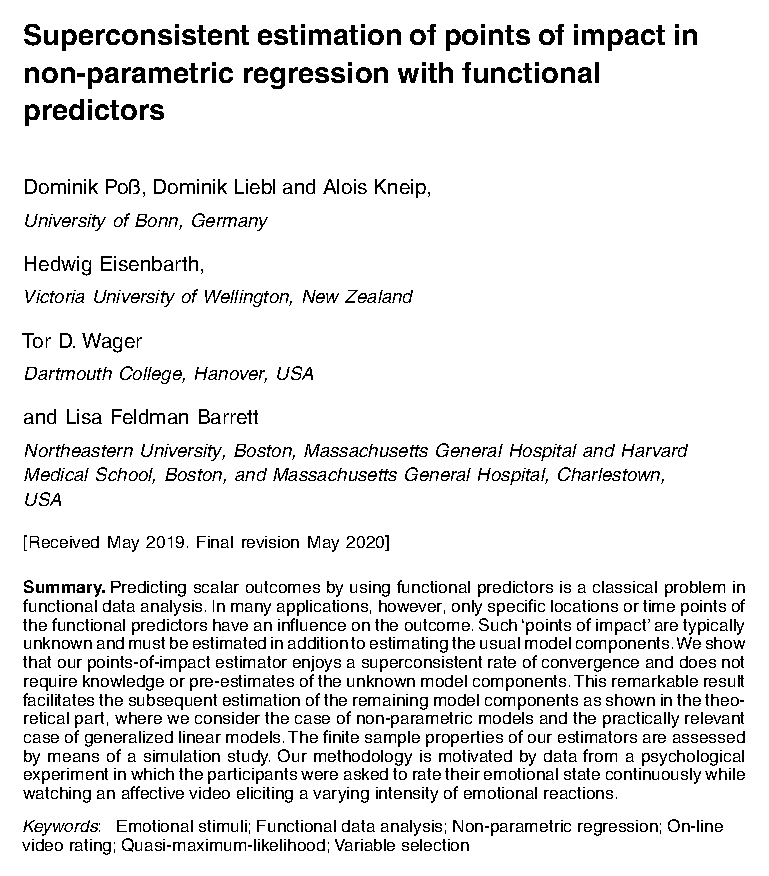
\includegraphics[width=0.45\textwidth]{files/paper-titlepage.pdf}}
\end{figure}
\end{frame}

\begin{frame}{The Setting}{Liebl (2020)}
\begin{figure}[ht]
    \centering
    \vspace{-1cm}
    
\includegraphics[width=0.55\textwidth]{files/drawing.pdf}
    \fbox{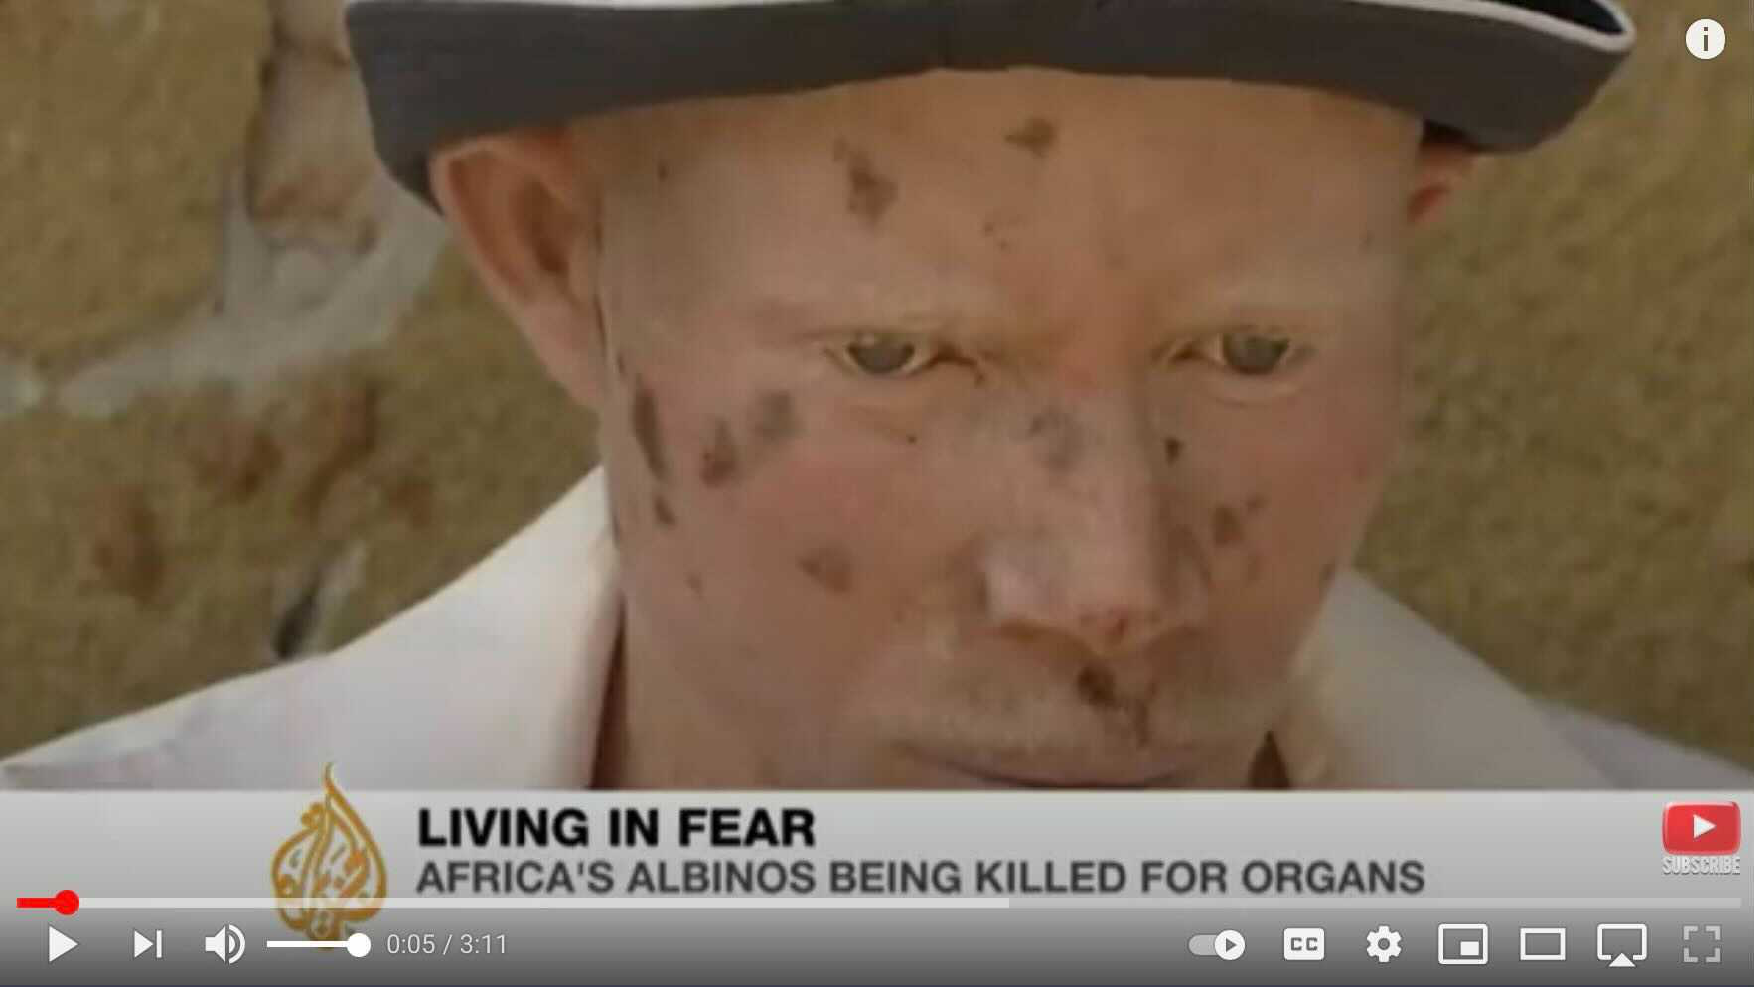
\includegraphics[width=0.35\textwidth]{files/video-snapshot.pdf}}
\end{figure}
\end{frame}

\begin{frame}{The Setting}
    \vspace{-1cm}
    \hspace{0.5cm}
    \begin{centering}
     \begin{tikzpicture}

         % time line
         \draw[line width=0.25mm, ->] (-3.75,0) -- (3.5,0) node [below] {};
         \draw (-3.25, -0.1) -- (-3.25, 0.1) node [below] {\shortstack{\\ \footnotesize Video Start}};
         \draw (2.5, -0.1) -- (2.5, 0.1) node [below] {\shortstack{\\ \footnotesize Video End}};

         % horizontal scale
         \draw[line width=0.25mm] (7, -3) -- (7, 3) node [above] {Sentiment};
         \foreach \x in {-3,-2,...,3}
            \draw (6.8, \x) -- (7.2, \x);

         \node[align=right] at (7.5, 0) {$0$};
         \draw[color=bonnblue, line width=0.3mm] (6.8, 1) -- (7.2, 1);

         % time-point
         \draw[line width=0.3mm, color=bonnblue] (-1, 0.1) -- (-1, -0.1);
         \node[] at (-1, -0.75) {\textcolor{bonnblue}{$\bm{\tau}$}};
         \draw[color=bonnblue, line width=0.3mm, ->] (-1, 0.25) .. controls (1, 1) and (3, 3) .. (5.5, 1) node [right] {\textcolor{bonnblue}{$\bm{X_i(\tau)}$}};

         \pause
         
         % outcome
         \draw[color=bonngrey, line width=0.3mm, ->] (2.5, -0.5) .. controls (2, -2) and (1.25, -2.2) .. (0, -2.5) node [left] {\textcolor{bonngrey}{$\bm{Y_i} \in \{0, 1\}$}};
         
     \end{tikzpicture}
 \end{centering}
\end{frame}


\newcommand{\brownianmotion}[5]{% points, advance, rand factor, options, end label
\draw[#4] (0,0)
\foreach \x in {1,...,#1}
{   -- ++(#2,rand*#3)
}
node[right] {#5};
}

\begin{frame}{The Data}{Regressors}
\pgfmathsetseed{1341}
\begin{centering}
\begin{tikzpicture}
    \draw[line width=0.25mm, ->] (0, -2) -- (0, 3);
    \draw[line width=0.25mm, ->] (-1, 0) -- (11, 0) node [below] {$t$};
    \brownianmotion{180}{0.05}{0.25}{color=bonnblue, line width=0.2mm}{$X_1(t)$}
    \brownianmotion{180}{0.05}{0.25}{color=bonnyellow, line width=0.2mm}{$X_2(t)$}
    \brownianmotion{180}{0.05}{0.25}{color=bonngrey, line width=0.2mm}{$X_3(t)$}
\end{tikzpicture}
\end{centering}
\end{frame}


\begin{frame}{The Problem}
\pgfmathsetseed{1341}
\vspace{-1cm}
\begin{tikzpicture}[scale=0.8]

    \draw[line width=0.25mm, ->] (0, -2) -- (0, 3);
    \draw[line width=0.25mm, ->] (-1, 0) -- (11, 0) node [below] {$t$};
    \brownianmotion{180}{0.05}{0.25}{color=bonnblue, line width=0.2mm}{$X_1(t)$}
    \brownianmotion{180}{0.05}{0.25}{color=bonnyellow, line width=0.2mm}{$X_2(t)$}
    \brownianmotion{180}{0.05}{0.25}{color=bonngrey, line width=0.2mm}{$X_3(t)$}
    
    \pause

    \draw[line width=0.3mm, color=red] (2, 4) -- (2, -3) node [right] {$\tau_1$};
    \draw[line width=0.3mm, color=red] (5, 4) -- (5, -3) node [right] {$\tau_2$};

    \pause

    \node[] at (12, 4) {$Y_i \simeq g\big(X_i(\tau_1), X_i(\tau_2)\big)$};

    \pause

    \node[circle, draw=red, minimum size=1mm, scale=0.9] (c1) at (2, 1.9) {};
    \draw[line width=0.3mm, color=red, ->] (c1) .. controls (3, 6) and (10, 6) .. (11.5, 4.5);

    \node[circle, draw=red, minimum size=1mm, scale=0.9] (c2) at (5, 2.6) {};
    \draw[line width=0.3mm, color=red, ->] (c2) .. controls (10, 2) and (12.5, 2.5) .. (13, 3.6);

\end{tikzpicture}
\end{frame}
